% soctepmlate unofficial - SOČ = Středoškolská odborná činnost - Czech competition
% Author: Vojtěch Boček
% Edit by: Jaroslav Páral
% Version: 2018-02-12
% Source code: https://github.com/RoboticsBrno/soctemplate/
% Base on: http://www.jcmm.cz/cz/sablona-soc.html
% License: CC BY 4.0

\documentclass{template/socthesis}

\usepackage{subcaption}
\usepackage{amsmath}
\usepackage{enumitem}


\addbibresource{text.bib}

\titlecz{Coopmaster - systém pro kontrolu a automatizaci kurníku}
\titleen{Coopmaster - system for coop control and automation}
\author{Jaroslav Němec}
\field{18}
\school{Střední škola a vyšší odborná škola aplikované kybernetiky}
\mentor{Ing. David Podzimek}
\mentorstatement{Ing. Davida Podzimka}
\newcommand{\mentorthanks}{Ing. Davidu Podzimkovi}

% Změňte, pokud se liší
%\region{Jihomoravský}
%\placefooter{Brno 2017}

\begin{document}

    \maketitle

    \makecopyrightstatement{V~Hradci Králové}

    \makethanks{Děkuji svému školiteli \mentorthanks{} za obětavou pomoc, podnětné připomínky a nekonečnou trpělivost, kterou mi během práce poskytoval.}

    \pagestyle{empty}

    \section*{Anotace}
    Ve své práci jsem se zabýval návrhem a realizací kompletního řešení pro malé i střední zemědělce a hospodáře, které má pomoci plnit běžné činnosti. Cílem této práce bylo vytvořit a realizovat systém pro kontrolu a automatizaci chovu hospodářských zvířat.

    \subsection*{Klíčová slova}
    programování, automatizace, zemědělství, neuronové sítě, python, mikroservisní architektura

    \vspace{20mm}

    \section*{Annotation}
    In my work, I have been involved in the design and implementation of a complete solution for small and medium farmers and homesteaders to help them carry out their day-to-day activities. The aim of this work was to design and implement a system for control and automation of livestock farming.

    \subsection*{Keywords}
    programming, automation, agriculture, neural networks, python, microservice architecture

    \newpage
    \pagestyle{plain}

    \tableofcontents % vysází obsah

    %%% Začátek práce
    \setcounter{figure}{0}
    \setcounter{table}{0}
    \newpage

    %%% Úvod
    \chapter{Úvod}
V dnešní době je populární využívat moderní technologie a umělou inteligenci v různých aplikacích jako například monitoring pohybu zákazníků v obchodech nebo ve formě textových modelů čímž je například známe ChatGPT. Zároveň dnes ubývá lidí, kteří by se chtěli zabývat staráním se o hospodářská zvýřata a tudíž je potřeba, aby něco zaujmulo jejich místo. Zároveň jsem sám člověk, který rád zkoumá nové věci v oblasti informatiky a velice ho baví automatizování nejrůznějších úloh. Na základě těchto faktů jsem se rozhodl vytvořit téma práci popisující využití moderních technologií při chovu hospodářských zvýřat. Nápad na tuto práci vznikl díky mojí babičce, která chová doma slepice. Když odjede na dovolenou, stávám se já tím, kdo se o ně musí starat. Slepice je třeba dojet ráno a večer zkontrolovat a spočítat. Tato činnost je časově náročná kvůli cestování a kolikrát i zbytečná, protože většinou se nic neděje. A vzhledem k tomu, že jsem povoláním informatik, budu toto práci věnovat tomu jaké je moje řešení automatizace babiččina chovu.
\newline
Práce se dělí na teoretickou a praktickou část. V teoretické části jsou popsány základní pojmy a principy, jež jsou důležité pro plné chápání práce. Praktická část popisuje konkrétní implementaci a nasazení asistenčního systému pro chov hospodářských zvýřat. Čtenář může využít znalosti, které nasbírá během čtení teoretické části a jež mu následně pomůže chápat praktická část, jako návod k realizaci vlastního systému dle jeho potřeb.
\newline
Svojí konkrétní implementaci jsem zaměřil na chov Kura domácího z výše popsaných osobních důvodů, a protože byl pro mě nejdostupnější testovací zvíře. Systém jsem realizoval mikroservisní architekturou a jednotlivé služby jsou psány v populárnímu jazyce Python. Jako GUI rozhraní je šikovně použit open source software pro chytrou domácnost Home Assistant.
\newline
Ukázkový běh aplikace je dostupný na url adrese https://coopmaster.jarousnemec.cz/ s přihlašovacími údaji do Home Assistanta uživatel: \textbf{visitor} a heslo: \textbf{Heslo1234}. Zdrojový kód k jednotlivým službám a konfiguraci Home Assistanta je dostupný na serveru github.com.


    %%% Jak psát
    \chapter{Jak psát}
Abychom mohli napsat odborný text jasně a srozumitelně, musíme splnit několik základních předpokladů\cite{vut-zkousky}:
\begin{itemize}
	\item musíme mít co říci,
	\item musíme vědět, komu to chceme říci,
	\item musíme si dokonale promyslet obsah,
	\item musíme psát strukturovaně.
\end{itemize}

\section{Musíme mít co říci}
Nejdůležitějším předpokladem dobrého odborného textu je myšlenka.
Je-li myšlenka dost závažná, tak přetrvá, i když je neobratně a zmateně podaná.
Chceme-li však myšlenku podat co nejvýstižněji a ušetřit tak čtenáři čas, musíme dodržet určité zásady, o~kterých pojednáme dále.

\section{Musíme vědět, komu to chceme říci}
Dalším důležitým předpokladem dobrého psaní je psát pro někoho.
Píšeme-li si poznámky sami pro sebe, píšeme je jinak než výzkumnou zprávu, článek, diplomovou práci, knihu nebo dopis.
Podle předpokládaného čtenáře se rozhodneme pro způsob psaní, rozsah informace a míru detailů.

\section{Musíme si dokonale promyslet obsah}
Jakmile víme, co chceme říci a komu, musíme si rozvrhnout látku.
Ideální je takové rozvržení, které tvoří logicky přesný a psychologicky stravitelný celek, ve kterém je pro všechno místo a jehož jednotlivé části do sebe přesně zapadají.
Jsou jasné všechny souvislosti a je zřejmé, co kam patří.

Abychom tohoto cíle dosáhli, musíme pečlivě organizovat látku.
Rozhodneme, co budou hlavní kapitoly, co podkapitoly a jaké jsou mezi nimi vztahy.
Diagramem takové organizace je graf, který je velmi podobný stromu, ale ne řetězci.
Při organizaci látky je stejně důležitá otázka, co do osnovy zahrnout, jako otázka, co z~ní vypustit.
Příliš mnoho podrobností může čtenáře právě tak odradit jako žádné detaily.

\section{Musíme začít psát strukturovaně}
Máme-li tedy myšlenku, představu o~budoucím čtenáři, cíl a osnovu textu, můžeme začít psát.
Při psaní prvního konceptu se snažíme zaznamenat všechny své myšlenky a názory vztahující se k~jednotlivým kapitolám a podkapitolám.
Každou myšlenku musíme vysvětlit, popsat a prokázat.
Hlavní myšlenku má vždy vyjadřovat hlavní věta a nikoliv věta vedlejší.


    %%% Slovo Romana
    \chapter{Slovo Romana}
Titulní strana v~takové podobě, v~jaké se vám dostala, je navzdory veškeré projevené snaze velice chatrná a proto vám radím příliš nezasahovat do její stavby, neboť by to mohlo zcela rozhodit pozice všech objektů.
Primární snahou bylo dosáhnout její netečnosti vůči příliš dlouhým jménům (doc.
RNDr.
Jana Šťastně Vdaná, Ph.D.), názvům práce a názvům škol.

I~v~sekci Prohlášení zkuste držet svého kreativního ducha na uzdě, abyste jej vzápětí uplatnili v~celém následujícím textu.
Struktura textu by měla být zhruba následující:

\begin{enumerate}
\item[$\bullet$] úvod
\item teorie
\item metodika
\item výsledky
\item diskuze
\item[$\bullet$] závěr
\end{enumerate}
nicméně není pevně daná a spoustě prací sluší i tematičtější způsoby dělení informací.

\section{Plovoucí objekty}
Všechna čest Microsoftu za postupnou konverzi Wordu z~textového procesoru v~sázecím software.
Jedna z~mnoha vlastností nových verzí je možnost přidání titulku k~plovoucímu objektu, jako bývá obrázek či tabulka.

\begin{figure}[h]
  	\centering
 	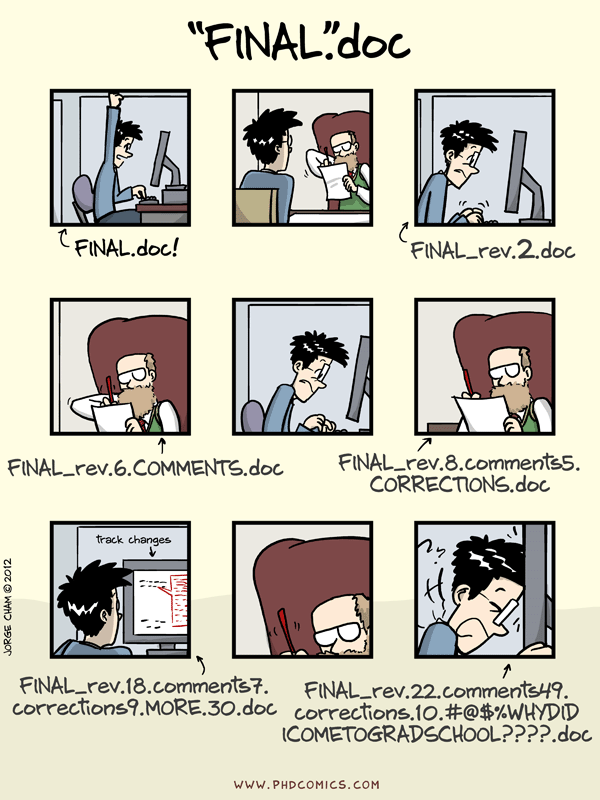
\includegraphics[width=200px]{img/final_doc.png}
 	\caption{Vás to nejspíše čeká taky.}
\end{figure}

\begin{table}[h]
  \centering
    \begin{tabular}{|l|l|}
    \hline
    Jednoduchá & tabulka \\ \hline
    o~& ničem \\
    \hline
    \end{tabular}
  \caption{Jak vidno, čísluje se separátně}
\end{table}

\begin{listedequation}[h]
$$L = - \frac{1}{4}F_{{\mu}v}F^{{\mu}v} + i \overline{\psi} \psi + \psi_i y_i \psi_j \phi + hc + |D_\mu\phi|^2 - V(\phi)$$
\caption{To je ale rovnice!}
\label{eq:hrnekeq}
\end{listedequation}

Vkládání popisků k~obrázkům a tabulkám lze zařídit poměrně snadno a intuitivně tlačítkem „Vložit titulek“ na kartě \It{Reference}.
U~rovnic se bohužel tento způsob uplatňuje jen velmi těžko, klasické vpravo zarovnané (1.1) lze pouze vykouzlit.
(Nápověda Microsoftu radí použít VBA makro, přívrženci Visual Basicu tedy nebudou mít problém.
Obávám se ale, že takových moc nebude.)

Využijte funkci „Vložit seznam obrázků“, která krom seznamu obrázků umí vkládat i seznam tabulek nebo rovnic.
Seznam obrázků v~práci být musí, i kdyby tam byl jen jeden obrázek.
Pro případ nejasnosti upřesňuji, že graf je považován za obrázek.

Co se dá naopak použít skvěle, jsou křížové odkazy.
Klepnutím na tlačítko „Křížový odkaz“ na kartě \It{Reference} mi umožní v~textu odkazovat na právě nějaký z~plovoucích objektů (či kapitolu, sekci, …) Proto nemám potíž zde uvést, že rovnice \autoref{eq:hrnekeq} odpovídá rovnici vyobrazené na hrnku na \autoref{fig:hrnek}, jen s~tím rozdílem, že na hrnku není formulována zcela správně.

\begin{figure}[h]
  	\centering
 	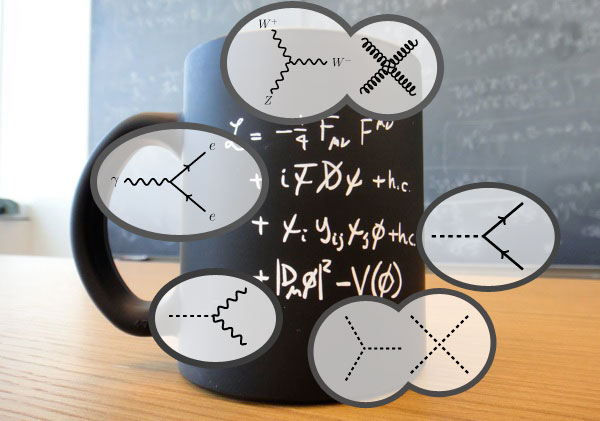
\includegraphics[width=\textwidth]{img/hrnek.jpg}
 	\caption{Hrneček ze Švýcarska}
 	\label{fig:hrnek}
\end{figure}

\section{Bibliografie}
Citovat je důležité (kruciální) a neméně důležité je citovat správně, a to v~ČR podle normy ČSN ISO 690 a ČSN ISO 690-2.
Důvod, proč ji tak mnoho lidí nedělá, je takový: Jedná se o~pěkně otravnou činnost\cite{citovani}.
To se však dá značně eliminovat použitím vhodného softwaru na správu a export citací.
Jaké máme možnosti?

Přímo českou normou se již dlouhou dobu zabývá projekt Citace.com umožňující zdarma získat toliko potřebné bibliografické záznamy.
Proces zkomfortňování šel až tak daleko, že si (např.) čtenáři registrovaní v~Moravské zemské knihovně (do 19 let vč.
zdarma) mohou nainstalovat do svého Wordu doplněk, který téměř vše zařídí za vás.

Pokud náhodou ještě nemáte a nemůžete mít účet v~Moravské zemské knihovně, nemusíte zoufat, i volně přístupná část nástrojů Citací.com má co nabídnout.
Na webu totiž můžete jednoduše vložit ISBN knihy nebo DOI (\It{Digital object identifier}) článku v~časopise a obratem vám bude vygenerována citace přesně podle normy, kterou můžete jednoduše zkopírovat do Wordu.
Číslování v~textu si však budete muset řešit sami.

Nicméně možnosti nekončí Citacemi.com, existuje celá řada dalších nástrojů (třeba EndNote).
Nebojte se požádat o~pomoc své školitele, sami si nejednou prošli stejným problémem a řešení s~velkou pravděpodobností našli.
Tak proč vynalézat kolo?

\subsection{Užitečné odkazy}
\begin{itemize}
    \item \url{http://www.citace.com}, \url{http://www.mzk.cz/}
	\item \url{http://www.boldis.cz/citace/citace1.pdf}
	\item \url{http://www.boldis.cz/citace/citace2.pdf}
	\item \url{https://sites.google.com/site/novaiso690/}
\end{itemize}

\section{Symboly, zkratky, slovníček}
Zkratky vysvětlujeme již při první zmínce v~textu, při jejich častějším výskytu může být praktické uvést ucelený seznam.
Totéž pak platí pro pojmy, které vysvětlujeme v~poznámce pod čarou\footnote{Poznámku pod čarou vložíme opět z~karty \It{Reference} tlačítkem \It{Vložit pozn.
pod čarou.}}: pokud jich je mnoho, vysázíme je i samostatně jako slovníček pojmů.

\section{Moudra závěrem}
Uvědomte si, že hlavním výstupem vaší roční činnosti nejsou data nebo zařízení, nýbrž právě odborný text, který má komisi SOČ ukázat, jak jste studované problematice porozuměli, jaký je váš vlastní přínos, jestli dokážete verbálně vystihnout vše podstatné a důležité.
\It{Formální a estetickou úpravou práce sdělujete komisi, jak moc vám záleží na tom, aby pro ně bylo čtení vaší práce příjemným či alespoň snesitelným zážitkem.}

Šablona je míněna jen jakýmsi odrazovým můstkem a nebojte, pořád na vás zbylo docela dost práce.
Bohužel víc, než jsem původně zamýšlel, protože sázení ve Wordu stále není žádný med a byla by jistě škoda ochudit vás o~četné nadávky na nesmyslnost jeho chování.
Všem počítačově zdatným jedincům pak doporučuji naučit se sazbu v~LaTeXu, je to dovednost, která se vám nikdy neztratí.

\begin{figure}[h]
  	\centering
 	
\includegraphics[width=\textwidth]{img/pulp.jpg}
 	\caption{Nejste v~tom sami.}
\end{figure}

Na závěr vám už poradím jen jedno: hledejte inspiraci.
Velmi dobře si pamatuji ten pocit, kdy sedíte nad prázdným dokumentem a přemýšlíte, co vlastně do té SOČky patří.
Kde začít? Co ještě zmínit a co už raději vynechat? Přitom máme všichni díky theses.cz na dosah stovky tisíc závěrečných prací starších kolegů z~vysokých škol.
Najděte si svůj vzor a jeďte podle něj, odborné posudky vedoucích a oponentů vám dokonce řeknou, co je správně a co nikoliv.

\vspace{\baselineskip}
\noindent Vědě zdar!

\vspace{\baselineskip}
\noindent \B{Roman Beránek} \\
\url{ischemy@gmail.com}


    %%% Závěr
    \newpage
\chapter*{Závěr}
\addcontentsline{toc}{section}{Závěr}

Závěrečná kapitola obsahuje zhodnocení dosažených výsledků se zvlášť vyznačeným vlastním přínosem studenta.
Povinně se zde objeví i zhodnocení z~pohledu dalšího vývoje projektu, student uvede náměty vycházející ze zkušeností s~řešeným projektem a uvede rovněž návaznosti na právě dokončené projekty.


    \newpage
    \printbibliography[title=Literatura]
    \addcontentsline{toc}{section}{Použitá Literatura}

    \listoffigures
    \addcontentsline{toc}{section}{Seznam obrázků}

    \listoftables
    \addcontentsline{toc}{section}{Seznam tabulek}

    \listoflistedequation
    \addcontentsline{toc}{section}{Seznam rovnic}

\end{document}
